As previously discussed, the size of the fuzzer's seed queue will quickly reach a large number (especially with the assistance of dynamic symbolic execution) when testing large-scale modern software. The seed queue should therefore be rearranged to find more paths in a given time budget.

We realized that different seed files in the queue have different affects on path discovery. For example in Figure~\ref{motivate-example}, suppose each input that triggers new behavior will be mapped to a specific dot. The fuzzer starts from an initial seed which is marked as red in this figure. The mutation results of this initial seed cover the black points as well as seed A and seed B. Then, in evolutionary fuzz testing, a test case will be picked up as the seed file for next round of mutation. 
Consider the choice between seed A and B in this figure.
 The \emph{distance}(e.g. Euclidean Distance) from the initial seed file to A is much shorter than B. 
  This means that A is more \textbf{\textit{similar}} to the initial seed file than B. So choosing A as the next seed file to mutate will only trigger two new paths (the blue area) as most of the mutated test cases are overlapped by what the initial seed has mutated (the gray area). However, because seed B has a longer distance from the initial seed than seed A, the coverage area of B (the brown area) will have less overlap by that of initial seed file than A. So choosing seed B will trigger more new behaviors than selecting seed A.

Based on this insight, we propose a seed selection method for the fuzzer based on the \textit{distance} between test cases.
Our method firstly maps each seed in the queue as a numerical vector. 
 Then each seed is assigned with a \emph{weight} value according to the distance from other test cases and its runtime information, which is then utilized as the criteria to determine which seed file should be scheduled as the next seed.
 
We investigate three popular distance measures, i.e., \textit{Euclidean Distance}, \textit{Cosine Similarity} and \textit{Jaccard Index}, as the distance metrics for calculating the \textit{weight} value for each seed. 
 In the following sections, we firstly review these three distance metrics and then explain how a test case is mapped to a numerical vector as well as the seed selection method.

\begin{figure}[!t]
\centering
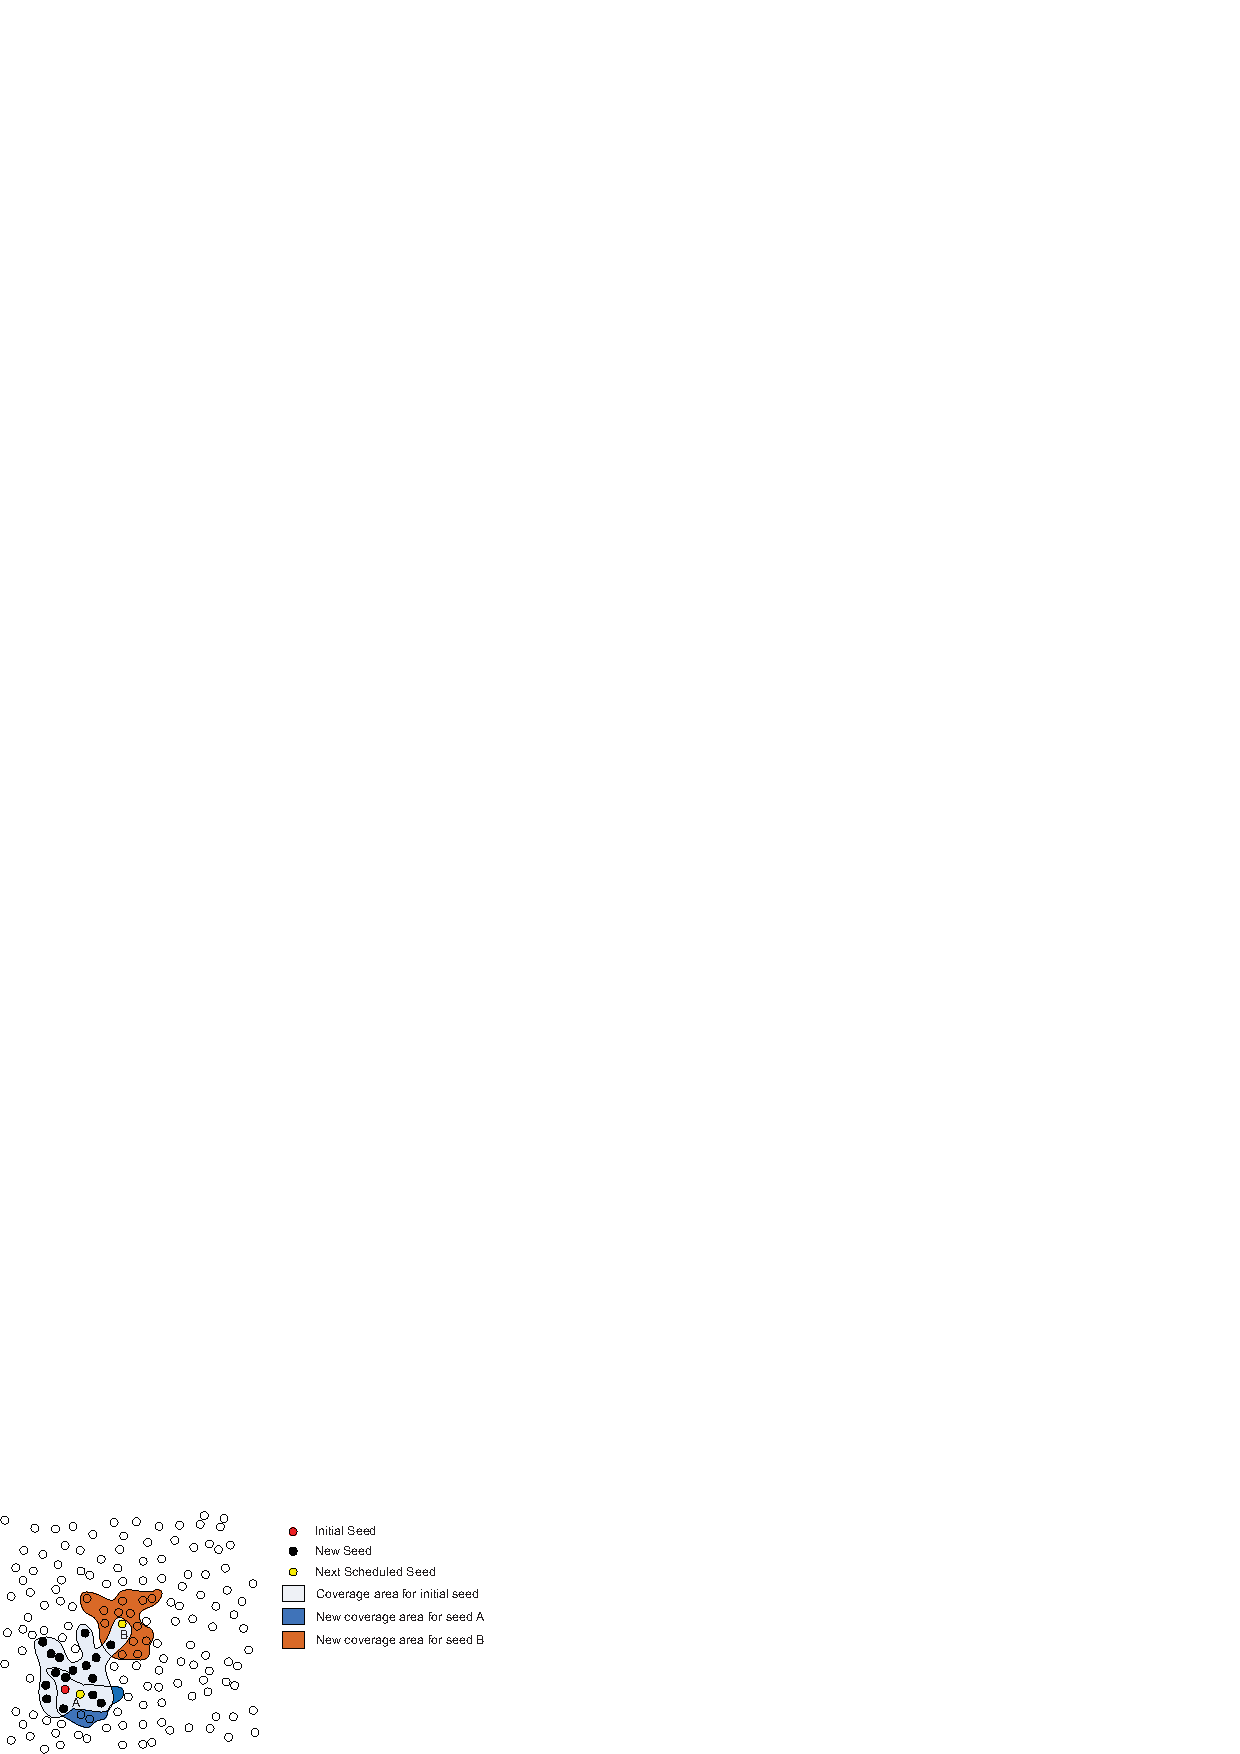
\includegraphics[width=0.5\textwidth]{figures/motivate-example.pdf} 
\caption{A motivating example.}\label{motivate-example}
\end{figure}

\subsection{Distance Metrics}
For two vectors $\mathit{X} = (x_1, x_2, \cdots, x_N)$ and $\mathit{Y} = (y_1, y_2, \cdots, y_N)$, the corresponding similarity metrics for \textit{Euclidean Distance}, \textit{Cosine Similarity} and \textit{Jaccard Index} are listed as follows.

\begin{enumerate}
\item Euclidean Distance (EU)

The Euclidean Distance between two vectors is defined as follows:
\begin{center}
$EU(\mathit{X}, \mathit{Y}) = \displaystyle \sqrt{\sum_{i=1}^{N} (x_i-y_i)^2}$
\end{center}

\item Cosine Similarity (CS)

The consine similarity between $\mathit{X}$ and $\mathit{Y}$ is defined as follows:

\begin{center}
$CS(\mathit{X}, \mathit{Y}) = \displaystyle \sqrt{\frac{\mathit{X}^T \cdot \mathit{Y}} {\| \mathit{X} \|\| \mathit{Y} \|}}$
\end{center}
where $\mathit{X}^T$ is a transposition of vector $\mathit{X}$ and $\| \mathit{X}\|$ is the Euclidean Distance of
vector $\mathit{X}$. Similarly, $\|\mathit{Y}\|$ is the Euclidean norm of vector $\mathit{Y}$. In essence, \textit{CS} is the cosine of the angle between $\mathit{X}$ and $\mathit{Y}$ in the N-dimensional space. For cosine similarly, the corresponding distance is defined as:

\begin{center}
$D(\mathit{X},\mathit{Y}) = 1 - CS(\mathit{X},\mathit{Y})$
\end{center}

\item Jaccard Index (JI)

The Jaccard Index between $\mathit{X}$ and $\mathit{Y}$ is defined as follows:

\begin{center}
$JI(\mathit{X}, \mathit{Y}) = \displaystyle \frac{\mathit{X} \cdot \mathit{Y}}{\mathit{X} \cdot \mathit{Y}+\omega(\|\mathit{X}\|^2+\|\mathit{Y}\|^2-2(\mathit{X} \cdot \mathit{Y}))}$
\end{center}

where $\mathit{X} \cdot \mathit{Y}$ is the inner product of $\mathit{X}$ and $\mathit{Y}$. 
When $\omega$ is equal to 1, the above formula is called Jaccard index and its corresponding distance is defined as follows:

\begin{center}
$D(\mathit{X},\mathit{Y}) = 1 - JI(\mathit{X},\mathit{Y})$
\end{center}

\end{enumerate}

\subsection{Seed Selection Method}
In order to measure the distances, all test cases should be mapped as numerical vectors. 
The mapping can be performed into both the input space and state space. Mapping into the input space cannot reflect the real relationship between test cases when considering the behavior of the target program. For example, as shown in Figure~\ref{distance-illusion}, multiple different inputs can steer the program to execute the same path. Specifically, considering the three test cases namely \texttt{A.jpeg}, \texttt{B.jpeg} and \texttt{C.jpeg} in this figure, suppose the corresponding contents are shown as follows:
\\
\\
\indent\texttt{A.jpeg}: \texttt{$\backslash$xFF$\backslash$xD8$\backslash$xAA$\backslash$xBB$\backslash$xCC$\backslash$xDD}

\texttt{B.jpeg}: \texttt{$\backslash$xFF$\backslash$xD8$\backslash$xDD$\backslash$xCC$\backslash$xBB$\backslash$xAA}

\texttt{C.jpeg}: \texttt{$\backslash$xFE$\backslash$xD8$\backslash$xAA$\backslash$xBB$\backslash$xCC$\backslash$xDD}
\\

\indent If we calculate the \textit{Euclidean Distance} between these three files directly in the input space, $ED_{AB}$ will be greater than $ED_{AC}$ because there are more different bytes between \texttt{A.jpeg} and \texttt{B.jpeg} than that of \texttt{A.jpeg} and \texttt{C.jpeg}. This means \texttt{A.jpeg} and \texttt{C.jpeg} are more similar (as shown in Figure~\ref{distance-illusion}) from the viewpoint of input space. 
However, for most of JPEG process programs, \texttt{A.jpeg} and \texttt{B.jpeg} will execute the same path, and \texttt{C.jpeg} will execute another path because \texttt{C.jpeg} is an illegal JPEG file (bad magic number). So from the viewpoint of the program, \texttt{A.jpeg} and \texttt{B.jpeg} are more similar than \texttt{A.jpeg} and \texttt{C.jpeg} even though \texttt{A.jpeg} and \texttt{C.jpeg} have only one bit difference. 
Since our objective is to maximize the coverage in the state space, we choose to map all the test cases as numeric vectors in the state space to calculate the distance.

In \cite{wang2015similarity}, all test cases are represented as a branch coverage vector $\mathit{V}=(v_1, v_2, \cdots, v_N)$, where $v_i$ is 0 means the branch is covered, otherwise 1. 
However, different test cases can affect different number of branches, so the mapped vectors may have different lengths which cannot be used directly for distance calculation. Meanwhile, it will be difficult to construct such vectors because obtaining all the branches and listing them \textit{orderly} in each vector to avoid obfuscation between vectors is nearly impossible for binary programs. 
In AFL \cite{online:afl}, the execution path information of each test case is stored as a \emph{Bitmap}. By checking the hit count of this bitmap, AFL determines whether some new behaviors are triggered. So as this bitmap contains enough information to reflect the characteristics of a test case from the viewpoint of the state space, we choose the bitmap as our mapped vector to mitigate the costly mapping in \cite{wang2015similarity}.

\begin{figure}
\centering
\includegraphics[width=0.3\textwidth]{figures/distance-illusion.pdf} 
\caption{An illusion for distance.}\label{distance-illusion}
\end{figure}

Based on the mapped bitmap vectors, the test case queue in the fuzzer is enhanced by assigning each test case with weight $W$, where $W$ is obtained by calculating the distance between every two test cases. Whenever a new seed file is found, the distance between this seed file and all the other files in the queue will be measured to calculate $W$. Meanwhile, the weight of all the other files in the queue will be updated according to the distance to the new seed file. 

Rather than selecting the seed file that has the longest distance to the current seed file (which is only a \emph{local optimum solution}), our search method selects the file that takes the longest average distance from all the other test cases as the next seed file. By doing this, we can achieve a \emph{global optimum solution} for this searching problem. The weight $W$ for test case $t_k$ is defined as follows:

\begin{center}
$W_k = \displaystyle\frac{1}{N} \sum_{i=0}^{N} D(t_i, t_k)$
\end{center}
where $D(t_i, t_k)$ denotes the distance between $t_i$ and $t_k$ based on the three distance measures mentioned before, and $N$ is the size of the test case queue. 

We also noticed that even though two test cases have the same $W$ value, they may have different power on finding new paths.
 This is because path coverage is not the only criteria for testing, and other runtime information, such as memory operations, can also be leveraged to prioritize test cases. 
 So we enhanced the weigh $W$ with memory coverage to achieve better prioritization result. The enhanced weight $\hat{W_k}$ for test case $t_k$ is defined as the following formula, where $M(t_k)$ denotes the number of memory cells that $t_k$ covers in byte.
\begin{center}
$\hat{W_k} = \displaystyle M(t_k) + \frac{1}{N} \sum_{i=0}^{N} D(t_i, t_k)$
\end{center} 